\documentclass[a4paper,UTF8]{article}
\usepackage{ctex}
\usepackage[margin=1.25in]{geometry}
\usepackage{color}
\usepackage{graphicx}
\usepackage{amssymb}
\usepackage{amsmath}
\usepackage{amsthm}
%\usepackage[thmmarks, amsmath, thref]{ntheorem}
\theoremstyle{definition}
\newtheorem*{solution}{Solution}
\newtheorem*{prove}{Proof}
\usepackage{multirow}
\usepackage{url}
\usepackage[colorlinks,urlcolor=blue]{hyperref}
\usepackage{enumerate}
\renewcommand\refname{参考文献}

%图片
\usepackage{subfigure}         
\usepackage{natbib}
\usepackage{float}
\usepackage{epstopdf}


%--

%--
\begin{document}
\title{\textbf{《计算机图形学》9月报告}}
\author{181860155 朱晓晴 \href{mailto:xxx@xxx.com}{heloize@126.com}}
\maketitle

\section{综述}
在9月提交中,主要完善了cg\underline{ }cli.py和cg\underline{ }algorithms.py两个模块。
在cg\underline{ }cli.py中,补充了对drawPolygon、drawEllipse等指令的解析。
在cg\underline{ }algorithms.py中,完成了绘制线段的所有算法(即draw\underline{ }line函数)
和绘制椭圆的算法(即draw\underline{ }ellipse函数)。


\section{算法介绍}
% 已完成或拟采用算法的原理介绍、自己的理解、对比分析等
\subsection{算法原理}

\subsubsection{绘制线段}
\textbf{要求:}根据给定两点$(x_0,y_0)$和$(x_1,y_1)$绘制线段。

绘制线段共需完成3种算法:Naive算法、DDA算法和Bresenham算法。
其中Naive算法已提供,9月提交中完成了DDA算法和Bresenham算法。

\textbf{DDA算法} \cite{ref1}

斜率$m=\frac{y_1-y_0}{x_1-x_0}$,
若$|m|<=1$,以$x_0<x_1$为例进行说明。
以单位间隔($\Delta x=1$)对$x$进行采样,并计算对应的$y$值:

$y_{k+1}=y_k+m\;(k=0,1,...)$

若$|m|>1$,以$y_0<y_1$为例进行说明。
以单位间隔($\Delta y=1$)对$y$进行采样,并计算对应的$x$值:

$x_{k+1}=x_k+\frac{1}{m}\;(k=0,1,...)$

\textbf{Bresenham算法} \cite{ref1}

将$(x_0,y_0)$作为第一个点,
计算决策参数的第一个值$p_0=2\Delta y-\Delta x$
($\Delta x=x_1-x_0$,$\Delta y=y_1-y_0$)。

若$|m|<=1$,以$m>0$且$x_0<x_1$的情况为例进行说明。
在每个$x_k$处进行检测:

$p_k<0$,下一个点为$(x_{k+1},y_k)$,
下一个决策参数$p_{k+1}=p_k+2\Delta y$;

$p_k\geqslant 0$,下一个点为$(x_{k+1},y_{k+1})$,
下一个决策参数$p_{k+1}=p_k+2\Delta y-2\Delta x$。

上述步骤共进行$\Delta x$次。

若$|m|>1$,以$m>0$且$y_0<y_1$的情况为例进行说明。
在每个$y_k$处进行检测:

$p_k<0$,下一个点为$(x_k,y_{k+1})$,
下一个决策参数$p_{k+1}=p_k+2\Delta x$;

$p_k\geqslant 0$,下一个点为$(x_{k+1},y_{k+1})$,
下一个决策参数$p_{k+1}=p_k+2\Delta x-2\Delta y$。

上述步骤共进行$\Delta y$次。


\subsubsection{绘制椭圆}
\textbf{要求:}根据给定的椭圆矩形包围框
左上角坐标$(x_0,y_0)$和右下角坐标$(x_1,y_1)$绘制椭圆。

\textbf{中点圆生成算法} \cite{ref1}

计算出椭圆中心$(x_c,y_c)$,长短轴径$r_x$和$r_y$。

(1)区域1中(|切线斜率|$\leqslant 1$)

计算得中心在原点的椭圆上的第一个点$(0,r_y)$,
计算区域1决策参数的初值
$p1_0=r_y^2-r_x^2r_y+\frac{r_x^2}{4}$。
在区域1每个$x_k$处,对决策参数进行检测:

$p1_k<0$,下一个点为$(x_{k+1},y_k)$,
下一个决策参数$p1_{k+1}=p1_k+2r_y^2x_k+3r_y^2$;

$p1_k\geqslant 0$,下一个点为$(x_{k+1},y_k-1)$,
下一个决策参数$p1_{k+1}=p1_k+2r_y^2x_k-2r_x^2y_k+2r_x^2+3r_y^2$。

循环直到$2r_y^2x\geqslant 2r_x^2xy$。

(2)区域2中(|切线斜率|$>1$)

取第一个点$(r_x,0)$,
计算区域2决策参数的初值
$p2_0=r_x^2-r_xr_y^2+\frac{r_y^2}{4}$。
在区域2每个$y_k$处,对决策参数进行检测:

$p2_k\leqslant 0$,下一个点为$(x_k,y_{k+1})$,
下一个决策参数$p2_{k+1}=p2_k+2r_x^2y_k+3r_x^2$;

$p2_k>0$,下一个点为$(x_k-1,y_{k+1})$,
下一个决策参数$p2_{k+1}=p2_k+2r_x^2y_k-2r_y^2x_k+2r_y^2+3r_x^2$。

循环直到$2r_y^2x<2r_x^2xy$。

最后,计算出其他三个象限中的点,
并将所有的点平移到中心为$(x_c,y_c)$的椭圆轨迹上。

\subsubsection{拟采用算法}
重置画布、保存画布和设置画笔颜色的功能在demo中已经实现,
9月提交则完成了绘制线段和绘制椭圆的功能,
剩余绘制多边形、绘制曲线、图元平移、图元旋转、图元缩放、裁剪线段
等功能待后续完成。

其中,
绘制多边形将采用DDA算法和Bresenham算法,
绘制曲线将采用Bezier算法和B-spline算法,
裁剪线段将采用Cohen-Sutherland算法和Liang-Barsky算法。


        
\subsection{对比分析}

\subsubsection{绘制线段}
如图1所示,向绘制线段的3种算法给定参数。
其中,Naive算法和DDA算法获得的参数完全一致,
Bresenham算法获得的参数为另两种算法参数向下平移10个像素。

绘制结果如图2所示,从上至下三条线段分别由Naive算法、DDA算法和Bresenham算法生成。
根据图2,易观察得Naive算法的结果与另两种算法的结果差异较大。
Naive算法不区分斜率绝对值小于1和大于1的情况,
同时浮点增量的连续叠加中取整误差的积累会使长线段所计算的像素位置偏离实际线段\cite{ref1}。
而DDA算法和Bresenham算法优化了上述两个问题,计算结果与实际线段更接近。
因此,图2中DDA算法和Bresenham算法结果无显著区别,而Naive算法的结果较前两者差异较大。

\begin{figure}[H]
    \centering
    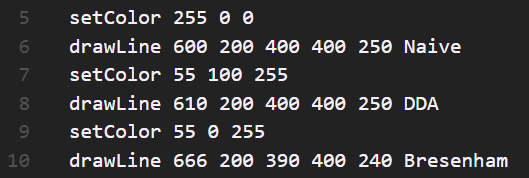
\includegraphics[width=5.3cm,height=1.8cm]{1.png}
    \caption{线段绘制指令}
\end{figure}

\begin{figure}[H]
    \centering
    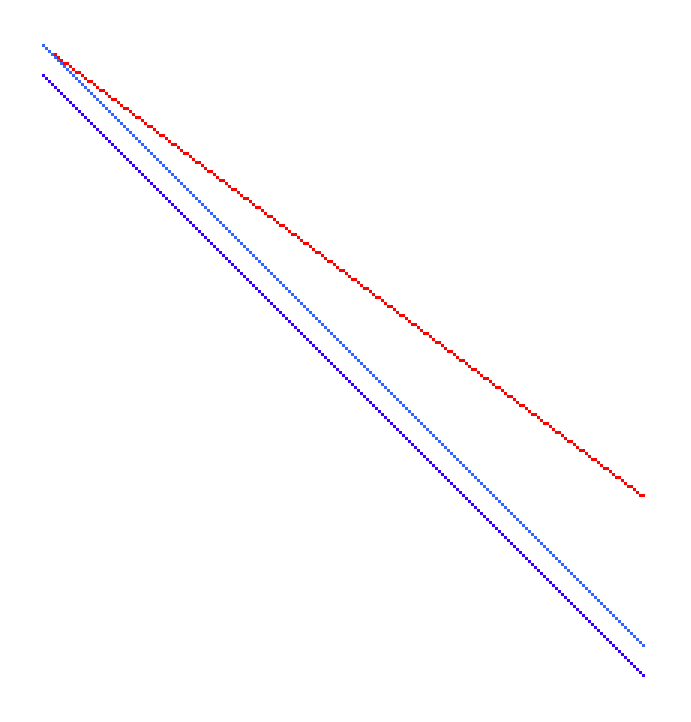
\includegraphics[width=4.6cm,height=4.8cm]{2.png}
    \caption{线段绘制算法比较}
\end{figure}



\subsubsection{绘制椭圆}
绘制椭圆采用了中点圆生成算法,
根据课本对中点圆生成算法的定义,
当取得区域1中的最后一个点,
不妨设其为$(x_a,y_a)$,
应根据$(x_a,y_a)$计算出区域2中决策参数的初值$p2_0$,
然后以单位间隔对$y$取样,
直到取到点$(r_x,0)$。
课本定义的中点圆生成算法计算出的结果如图3所示:

\begin{figure}[H]
    \centering
    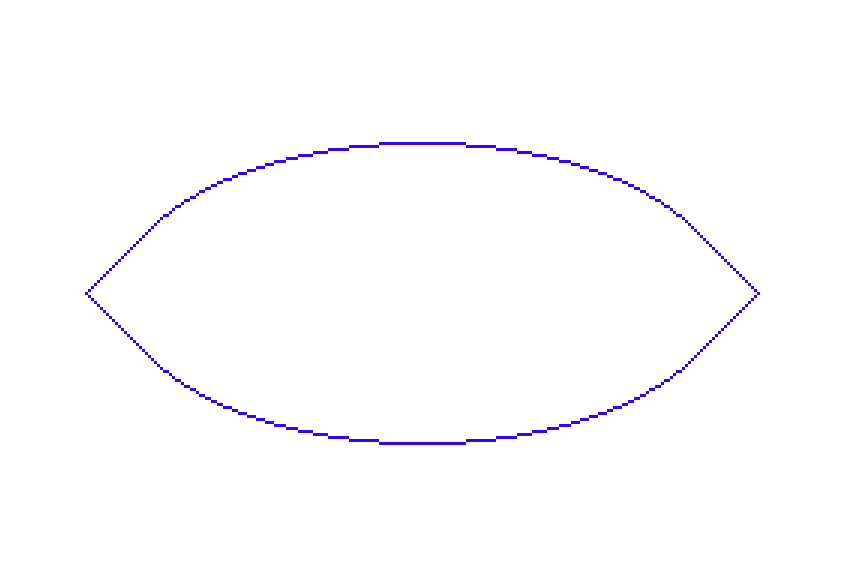
\includegraphics[width=4.3cm,height=2.8cm]{3.png}
    \caption{课本中点圆生成算法结果}
\end{figure}

分析结果错误的原因,区域2以$(x_a,y_a)$为起点,
并不能确保最后一个点取到$(r_x,0)$。
参考相关博客\cite{ref2}后,
将区域2的算法修改为:
以$(r_x,0)$为起点,计算决策参数的初值$p2_0$,
并按照2.1.2中的算法计算,直到切线斜率绝对值大于等于1。
上述算法计算出的结果如图4所示:

\begin{figure}[H]
    \centering
    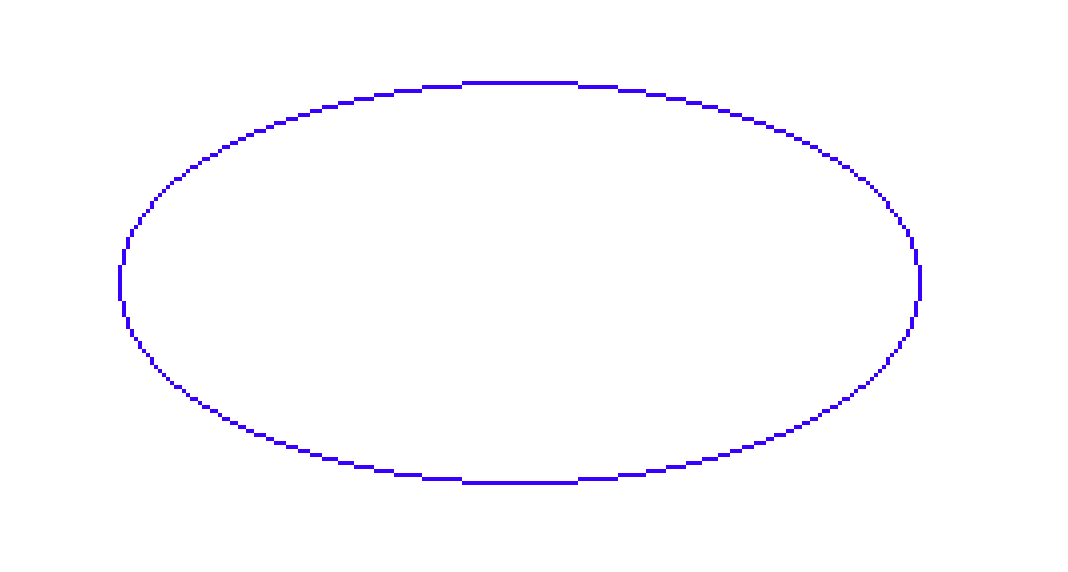
\includegraphics[width=4.3cm,height=2.7cm]{4.png}
    \caption{优化后的中点圆生成算法结果}
\end{figure}



\section{系统介绍}
% 已完成或拟采用的系统框架、交互逻辑、设计思路等
\subsection{交互逻辑}
目前,系统沿用demo的交互逻辑,即命令行和可视化界面两种运行方式。

以命令行方式运行时,
系统逐行读取指令文件,解析指令
并调用cg\underline{ }algorithms.py模块中的相关算法。

以可视化界面运行时,通过鼠标事件获取所需参数,
调用cg\underline{ }algorithms.py模块中的相关算法,
再以可视化方式直接呈现结果。

\subsection{设计思路}
后续,在完成要求的功能后,将着重优化图形界面。
目前,计划在图形界面中做出以下修改:

(1)对用户隐藏图元序号,直接通过鼠标操作选中图元,并对图元进行编辑;

(2)优化颜色设置方式,通过显示调色盘简化用户设置颜色的过程;

(3)添加可绘制的图元类型,如填充图元、虚线等。


\section{总结}
9月提交中,运用了目前已讲到图形学基础知识,
并自学了解了绘制图元的若干算法。
通过实现绘制线段和绘制椭圆的算法,
加深了对图形显示原理的理解。
但目前对图形界面的理解较浅,
尚未基于demo的图形界面做出显著改动,
后续将着重优化图形界面,
使得整个图形学系统功能更为强大,
使用更为简易。

\bibliographystyle{plain}
%"xxx" should be your citing file's name.
\begin{thebibliography}{99}
% 注明在实现作业过程中使用的参考资料,包括技术博客等
\bibitem{ref1} 孙正兴等. 计算机图形学教程[M]. 机械工业出版社, 2006.
\bibitem{ref2} cumtv80668. 中点画椭圆算法. CSDN, 2020.

链接:https://blog.csdn.net/cumtv80668/article/details/107792162
\end{thebibliography}

\end{document}